\documentclass[10pt]{article}

\usepackage{mathtools, amsfonts, bm}
\usepackage{microtype}
\usepackage[utf8]{inputenc}
\usepackage[top = 1.0in, left = 1.75in, right = 0.75in, bottom = 0.75in]{geometry}
\usepackage{booktabs}
\usepackage{graphicx}
\usepackage{xcolor}
\usepackage{tabularx}
\usepackage{tikzsymbols}
\usepackage[hidelinks]{hyperref}

\usepackage[explicit]{titlesec}
\titleformat{\section}[runin]{\bfseries}{}{0em}{
    \llap{
        \smash{
            \begin{tabularx}{0.85in}{r}
                #1 
            \end{tabularx}
        }
    }
}[\leavevmode\hspace*{\dimexpr-\fontdimen2\font-\fontdimen3\font}]

\usepackage{fancyhdr}
\pagestyle{fancy}
\fancyhf{}
\rhead{\thepage}
\renewcommand{\headrulewidth}{0pt}

\usepackage{lipsum}

%' ============================================================================================================================================================
%' ============================================================================================================================================================

\begin{document}

\newcommand{\mytitle}{Homework 1}
\newcommand{\myauthor}{Aiden Kenny}
\newcommand{\myclass}{STAT GR5205: Linear Regression Models}
\newcommand{\myschool}{Columbia Univeristy}
\newcommand{\mydate}{September 21, 2020}
\begin{flushright}
    \textbf{\mytitle}\\[0.5em]
    \textsl{\myauthor}\\
    \textsl{\myclass}\\
    \textsl{\myschool}\\
    \textsl{\mydate}
\end{flushright} \vspace{1em}

%' ============================================================================================================================================================
\section{Question 1} \noindent
% We will first read in the data using the \verb|data.table| package, and we will make our
% plots using the \verb|ggplot2| package.
% \begin{verbatim}
% library(data.table)
% library(ggplot2)
% cm <- fread(input = 'data/copier_maintenance.txt')
% \end{verbatim}
\begin{figure}[h]
    \centering
    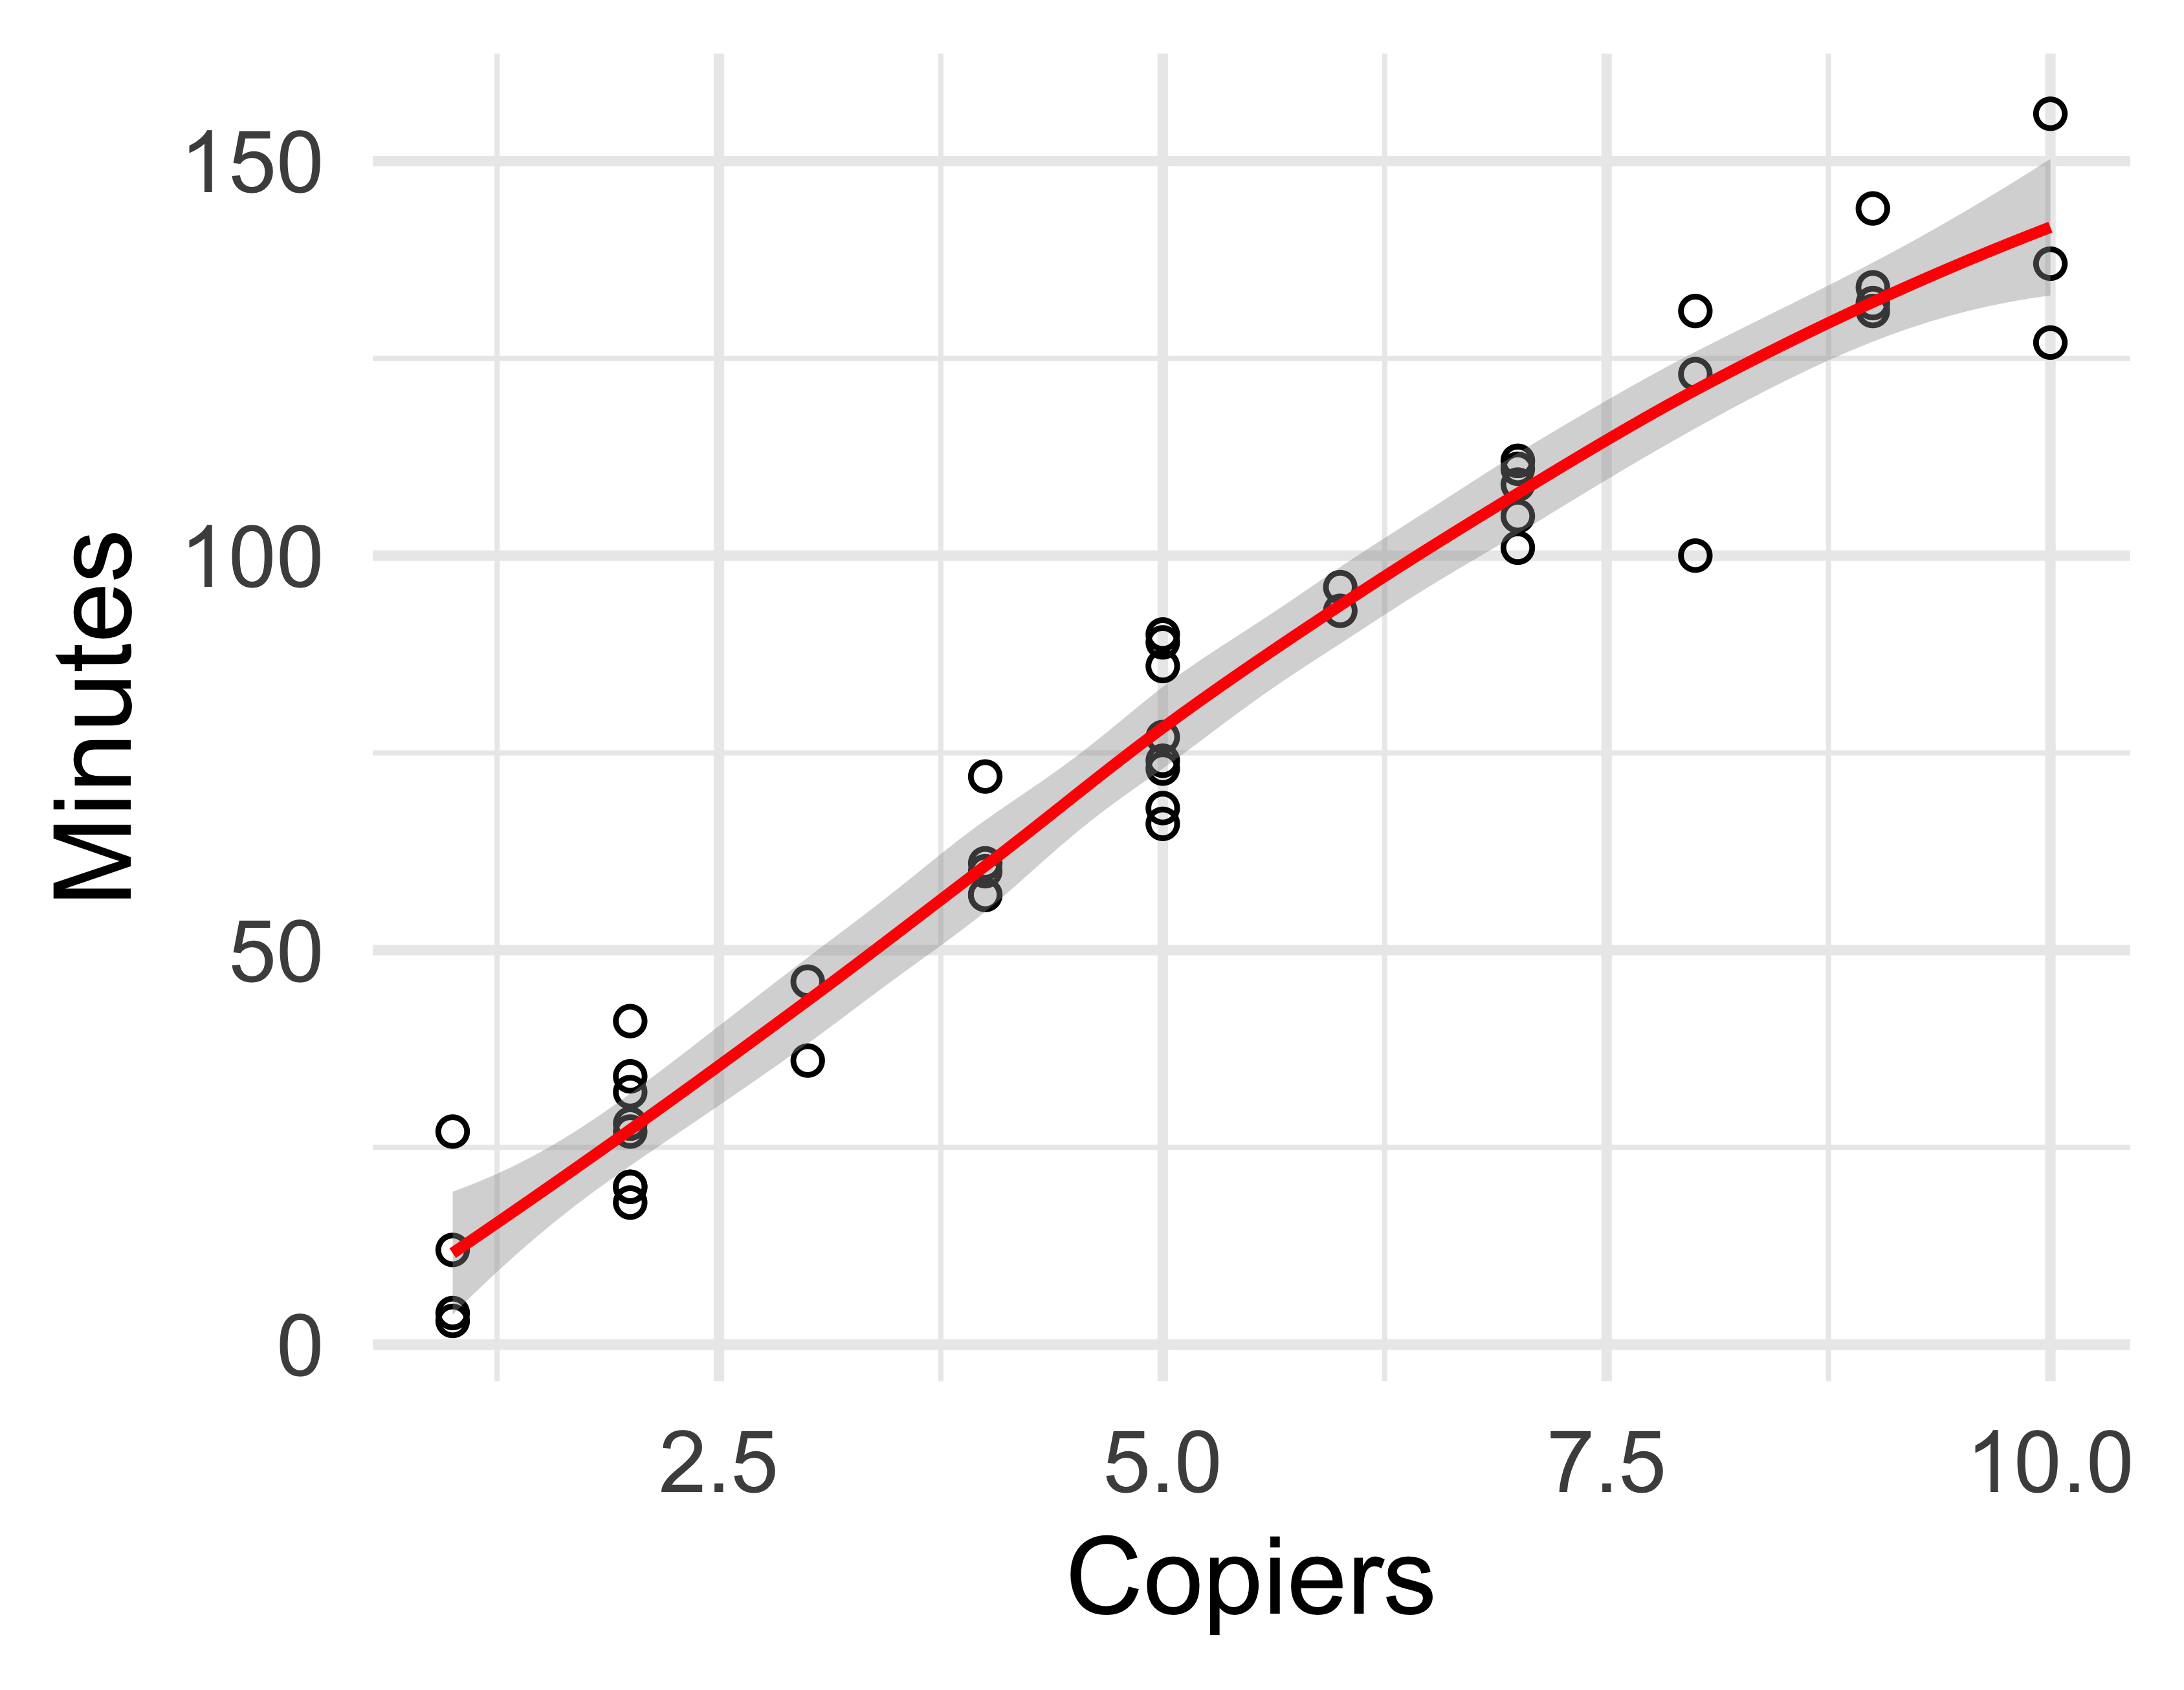
\includegraphics[width = 0.45\textwidth]{../img/q01_lowess.png}
    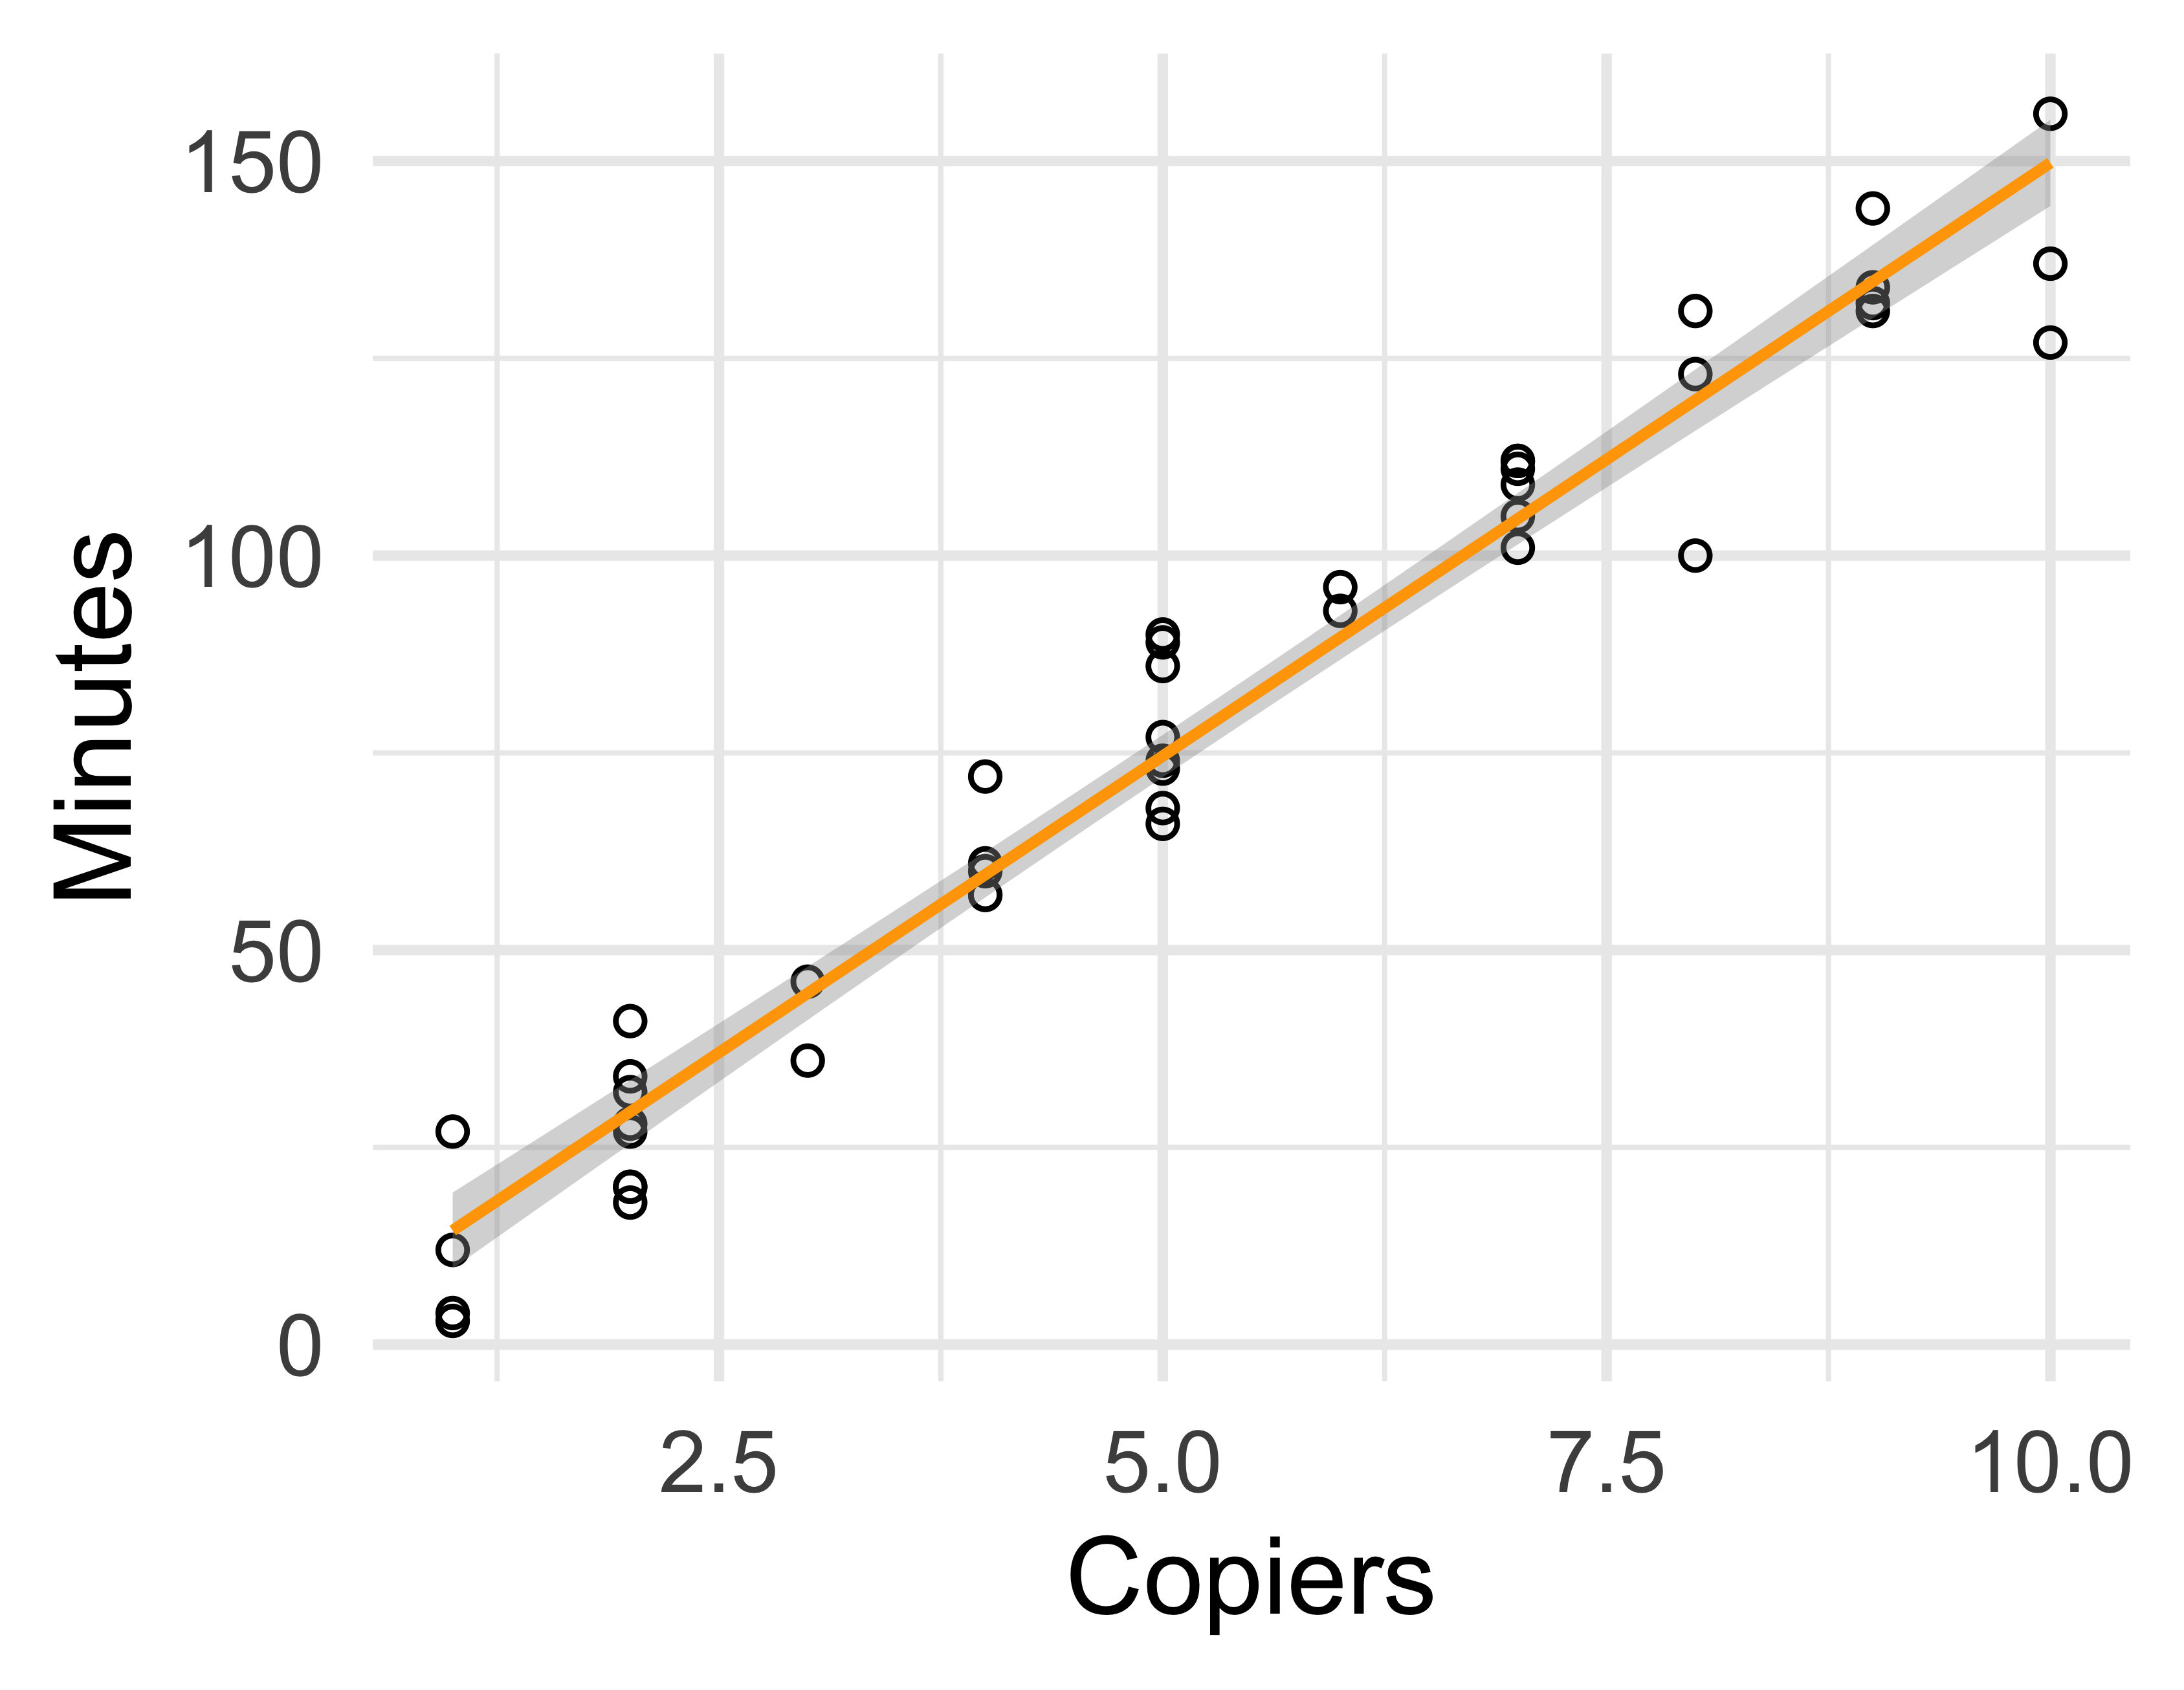
\includegraphics[width = 0.45\textwidth]{../img/q01_linear.png}
    \caption{Left: applying a LOWESS smoother to a scatterplot of the data. Right: 
    plotting the linear regression model to the scatterplot.}
    \label{q01_fig}
\end{figure} 
\begin{itemize}
    \item[(a)] Not sure what she wants here, ask more about LOWESS smoothers.
    \item[(b)] Using \texttt{R}, our estimated coefficients are given by \(\hat{\beta}_0 = -0.5801567\)
    and \(\hat{\beta}_1 = 15.0352480\), and so our estimated linear regression function is given by
    \[\hat{Y} = -0.5801567 + 15.0352480 \cdot X.\] The estimated linear regression model has been 
    overlayed on a scatterplot of the data in the right plot in Figure \ref{q01_fig}, and the 
    estimated function seems to fit the data well. The general trend, where an increase in number of 
    copiers results in an increased number of minutes on call, is captured by the model.
    \item[(c)] \(\hat{\beta}_1\) can be interpreted as follows. If the number of copiers serviced during
    a call increased by one, the total number of minutes of the call is expected to \textit{increase} by 
    \(15.0352480\) minutes. 
    \item[(d)] \(\hat{\beta}_0\) can be interpreted as follows. If there are zero copiers serviced during 
    a call, then we can expect the call to last for, on average, \(-0.5801567 \) minutes. This does \textit{not}
    provide any useful or relevant information; a call cannot ever have negative time, and a customer would never
    call if they did not have any copiers to service (where \(X = 0\)).
    \item[(e)] 
    \item[(f)] 
    \item[(g)] Using \texttt{R}, we can see that the residuals sum to 0; this is easy to do since the residuals are
    are included in the fitted model. We can think of \(Q\) as a \textit{function} 
    of \(\beta_0\) and \(\beta_1\), and we want to find the values of \(\beta_0\) and \(\beta_1\) that minimize \(Q\).
    The observed residuals \(e_i\), when plugged into \(Q\), give the smallest value of \(Q\) that can possibly be obtained. 
    Let \(\bm{\varepsilon} = (\varepsilon_1, \ldots, \varepsilon_n)^T\) be the random vector containing the \(n\) 
    residuals, and let \(\mathbf{e} = (e_1, \ldots, e_n)^T\) be the \(n\) realized residuals from \(\hat{\beta}_0\)
    and \(\hat{\beta}_1\). Using this 
    notation, we have \(Q = \| \bm{\varepsilon} \|_2^2\), and \[\| \mathbf{e}\|_2^2 = \min \|\bm{\varepsilon}\|_2^2 = \min Q.\]

\end{itemize}

%' ============================================================================================================================================================
\section{Question 2} \noindent
fafad

%' ============================================================================================================================================================
\section{Question 3} \noindent
The coefficients for the estimated linear regression function \(\hat{Y} = \hat{\beta}_0 + \hat{\beta}_1 \cdot X\) are
given by \[\hat{\beta}_1 = \frac{\sum_{i=1}^n (x_i - \bar{x})(y_i - \bar{y})}{\sum_{i=1}^n(x_i - \bar{x})^2}\]

%' ============================================================================================================================================================
\section{Question 4} \noindent
blah blah balh

\end{document}